% !TEX root = ../main.tex
\chapter{Fluiddynamikk}
\intro{... }

\spm{}{%
\item Hva er et fluid, og hva skiller det fra et fast stoff?
\item Hva bestemmer trykket i en væske?
\item Hva er oppdrift, og hvorfor flyter noen ting mens andre synker?}
\newpage

\section{Introduksjon til Fluidfysikk}

Fluidfysikk handler om studiet av fluider, som inkluderer både væsker og gasser. Et fluid er et materiale som kan flyte og tilpasse seg formen til beholderen det er i. I motsetning til faste stoffer, som har en fast form og volum, kan fluider lett endre form og tilpasse seg omgivelsene.\\

Væsker, som vann, har et bestemt volum, men kan flyte og tilpasse seg formen til beholderen sin. De har høyere tetthet enn gasser, og molekylene i en væske er relativt tettpakket, men de kan fortsatt bevege seg rundt hverandre. Gasser, som luft, har verken en fast form eller et fast volum. Gasser vil utvide seg og fylle hele volumet til beholderen de er i, og molekylene i en gass har mye større bevegelsesfrihet enn i en væske.

\subsection{Massettethet}

Massetetthet, også kjent som tetthet, er et mål på hvor mye masse som er pakket inn i et gitt volum av et stoff. Tettheten avgjør om et objekt vil synke eller flyte i et fluid, og den varierer mellom forskjellige materialer. For eksempel har metall en høyere tetthet enn tre, noe som forklarer hvorfor metall synker i vann mens mange tresorter flyter.

Tetthet er en viktig egenskap i både fysikk og ingeniørfag fordi den gir informasjon om hvordan ulike materialer oppfører seg når de påvirkes av krefter som tyngdekraft. Enheten for massetetthet er vanligvis kg/m\(^3\) eller g/cm\(^3\).

\defn{Massetetthet}{
    Massetetthet \( \rho \) kan uttrykkes som:
    \begin{align}
        \rho = \frac{m}{V}
    \end{align}
    hvor \( m \) er massen til stoffet og \( V \) er volumet. Massetettheten angir hvor mye masse som finnes per volumenhet.
}


\begin{table}[h!]
    \centering
    \begin{tabular}{|c|c|}
        \hline
        \textbf{Stoff} & \textbf{Tetthet \( \rho \) (\(10^3\) kg/m\(^3\))} \\
        \hline
        Gull & 19.3 \\
        \hline
        Stål & 7.85 \\
        \hline
        Vann & 1.0 \\
        \hline
        Luft & 0.0012 \\
        \hline
        Vanndamp & 0.0006 \\
        \hline
    \end{tabular}
    \caption{Massetetthet \( \rho \) til forskjellige stoffer, angitt i \( 10^3 \) kg/m\(^3\).}
    \label{tab:massetetthet}
\end{table}

\exm{Massetetthet av 1 liter vann}{
Hva er massen til 1 liter vann?

\textit{Løsning:} \\
Vi vet at massetetthet \( \rho \) er definert som massen \( m \) per volum \( V \):
\[
\rho = \frac{m}{V}
\]
For å finne massen \( m \), omformer vi formelen slik at
\[
m = \rho \cdot V
\]

Siden vi har oppgitt volumet som \( V = 1 \, \text{L} \), konverterer vi dette til kubikkmeter:
\[
1 \, \text{L} = 1 \, \text{dm}^3 = 1 \times 10^{-3} \, \text{m}^3
\]

Nå setter vi inn verdiene med \( \rho = 1.0 \times 10^3 \, \text{kg/m}^3 \) og \( V = 1 \times 10^{-3} \, \text{m}^3 \):
\[
m = (1.0 \times 10^3 \, \text{kg/m}^3) \times (1 \times 10^{-3} \, \text{m}^3)
\]
\[
m = 1.0 \, \text{kg}
\]

Massen til 1 liter vann er dermed \( 1.0 \, \text{kg} \).
}



\subsection{Trykk}

Trykk er definert som kraften som virker vinkelrett på en overflate per arealenhet. Det beskriver hvor mye kraft som påføres en bestemt flate, og det oppstår når molekyler i et fluid kolliderer med overflaten. Trykk måles ofte i enheter av pascal (Pa), hvor \( 1 \, \text{Pa} = 1 \, \text{N/m}^2 \).

\defn{Trykk}{
    Trykket \( p \) i et fluid er gitt ved:
    \begin{align}
        p = \frac{F}{A}
    \end{align}
    hvor \( F \) er kraften som virker vinkelrett på overflaten, og \( A \) er arealet til overflaten. Trykk måler kraft per arealenhet og uttrykkes vanligvis i pascal (Pa).
}

Trykk beskriver kraften som virker vinkelrett på en overflate per arealenhet. Det er en skalar størrelse, noe som betyr at trykk kun har en størrelse, men ingen retning som en vektor.\\

SI-enheten for trykk er pascal (Pa). En pascal tilsvarer én newton per kvadratmeter:
\[
1 \, \text{Pa} = 1 \, \text{N/m}^2
\]
En newton (N) er definert som kraften som gir en masse på 1 kg en akselerasjon på 1 m/s\(^2\), altså:
\[
1 \, \text{N} = 1 \, \text{kg} \cdot \text{m/s}^2
\]
Dette betyr at trykk også kan uttrykkes som \( 1 \, \text{Pa} = 1 \, \text{kg} \cdot \text{m}^{-1} \cdot \text{s}^{-2} \).\\


På mikroskopisk nivå kan trykk forstås som resultatet av at gassmolekyler kolliderer med veggene i en beholder. Hvert molekyl utøver en liten kraft på veggen når det treffer den, og summen av alle disse kollisjonene per arealenhet gir opphav til trykket i beholderen.

\begin{figure}[H]
    \centering
    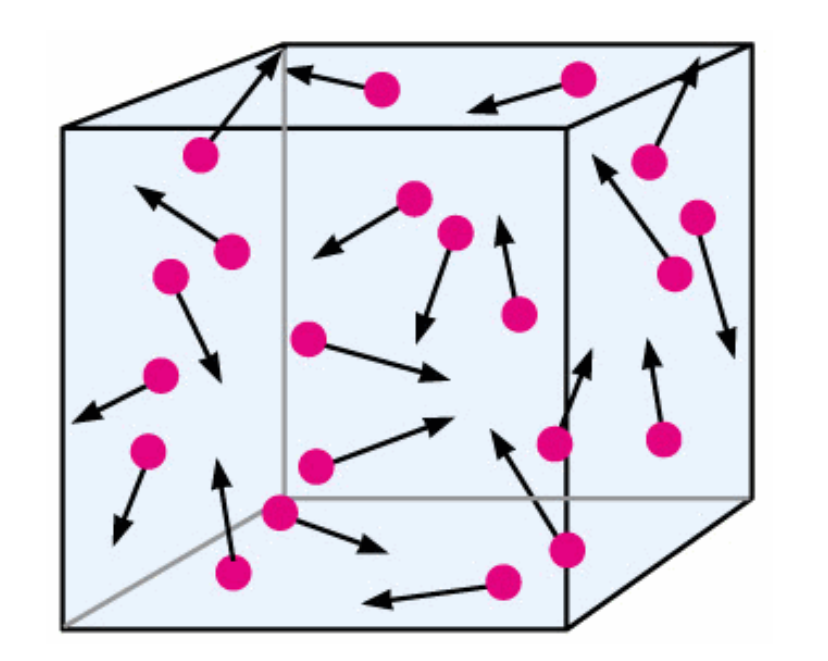
\includegraphics[width=0.6\textwidth]{Images/Kapittel4:Fluiddynamikk/Trykk.png}
    \caption{Trykk i gassbeholder}
    \label{fig:Trykk}
    \end{figure}


\section{Trykk i væsker}

Trykk i væsker oppstår som følge av vekten av væsken over et gitt punkt og de kreftene som væsken utøver på overflatene rundt seg. Dette trykket avhenger av væskens tetthet \( \rho \), dybden \( h \), og tyngdeakselerasjonen \( g \). Vi kan analysere væsketrykket ved å bruke to forskjellige elementer: et horisontalt væskeelement og et vertikalt væskeelement.

\subsection{Horisontalt væskeelement}
I et horisontalt væskeelement er trykket likt i alle retninger, forutsatt at væsken er i ro. Dette skyldes at væsker alltid fordeler kreftene jevnt i et horisontalt plan når de ikke er i bevegelse. Dersom trykket ikke var likt, ville væsken begynne å strømme fra områder med høyt trykk til områder med lavt trykk. Derfor gjelder:
\[
p_1 = p_2 \quad \text{(i et horisontalt væskeelement i ro)}.
\]

Men dersom væsken er i bevegelse, kan trykket variere i horisontal retning. For eksempel, i et rør hvor arealet av røret endrer seg, vil væsken begynne å strømme, og trykket blir forskjellig i de ulike delene av røret. Dette skyldes at væskens hastighet endres når røret innsnevres eller utvides, noe som påvirker trykket. 

\begin{figure}[H]
    \centering
    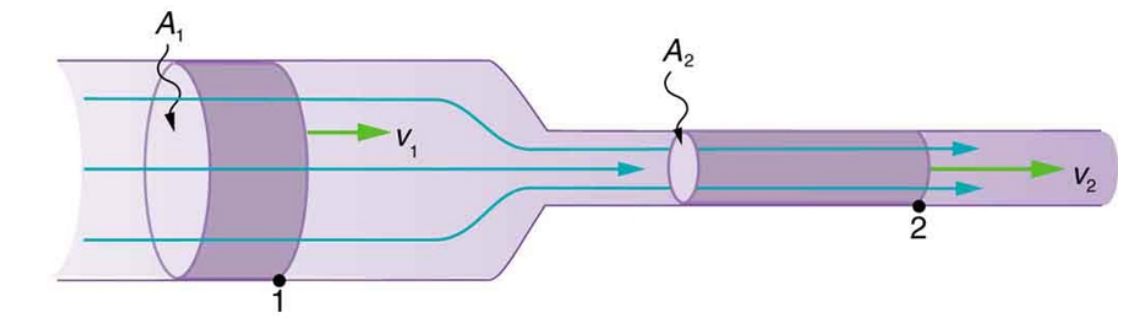
\includegraphics[width=0.8\textwidth]{Images/Kapittel4:Fluiddynamikk/rør_ulikt_trykk.png} 
    \caption{Et rør arealet reduseres fra \( A_1 \) til \( A_2 \). Trykket øker fra \( A_1 \) til \( A_2 \) når væsken passerer gjennom røret.}
    \label{fig:roer_variabelt_areal}
\end{figure}


Dersom røret derimot har samme areal langs hele lengden og er horisontalt, vil trykket være det samme langs hele røret, fordi væsken beveger seg med konstant hastighet, og det er ingen høydeforskjell som kan endre trykket.

\defn{Trykk i horisontalt væskeelement}{
    I et horisontalt væskeelement i ro gjelder:
    \begin{align}
        p_1 = p_2
    \end{align}
    hvor \( p_1 \) og \( p_2 \) er trykkene i forskjellige punkter på samme horisontale nivå. Dersom væsken strømmer og rørets areal endrer seg, vil trykket kunne variere.
}

\textbf{Hydrostatisk trykk:}  
Når vi beveger oss nedover i væsken, øker trykket på grunn av vekten av væsken over et gitt punkt. Det hydrostatiske trykket \( p \) ved en viss dybde \( h \) kan uttrykkes som:

\defn{Hydrostatisk Trykk}{
    Trykket \( p \) i en væske i ro på grunn av vekten av væsken over et punkt er gitt som:
    \begin{align}
        p = \rho g h
    \end{align}
    hvor \( \rho \) er væskens tetthet (\( \text{kg/m}^3 \)), \( g \) er tyngdeakselerasjonen (\( 9.81 \, \text{m/s}^2 \)), og \( h \) er dybden (\( \text{m} \)).
}

Det hydrostatiske trykket avhenger bare av dybden \( h \), væskens tetthet \( \rho \), og tyngdeakselerasjonen \( g \), og er uavhengig av væskeelementets horisontale størrelse.


\subsection{Vertikalt væskeelement}
I et vertikalt væskeelement virker vekten av væsken, som gir opphav til det hydrostatiske trykket. Kreftene som virker på dette væskeelementet inkluderer trykket \( p_1 \) på toppen, trykket \( p_2 \) på bunnen, og tyngdekraften på væskeelementet.

\defn{Trykkdifferanse i vertikalt væskeelement}{
    For et væskeelement i ro gjelder:
    \begin{align}
        p_2 - p_1 = \rho g h
    \end{align}
    hvor \( p_2 \) er trykket ved bunnen av elementet, \( p_1 \) er trykket ved toppen, og \( h \) er høyden til væskeelementet.
}

I en væske som er i ro, vil trykket øke med dybden på grunn av vekten av væsken over punktet. Dette trykket avhenger av væskens tetthet, tyngdeakselerasjonen, og dybden under overflaten. Dersom det også er et ytre trykk \( p_0 \) på væskeoverflaten, kan det totale trykket ved en dybde \( h \) uttrykkes som:

\defn{Trykk i et vertikalt væskeelement}{
    Trykket \( p(h) \) i en væske som er i ro er gitt som:
    \begin{align}
        p(h) = p_0 + \rho g h
    \end{align}
    Her er \( p_0 \) det ytre trykket ved væskeoverflaten, \( \rho \) er tettheten til væsken (\( \text{kg/m}^3 \)), \( g \) er tyngdeakselerasjonen (\( 9.81 \, \text{m/s}^2 \)), og \( h \) er dybden i væsken (\( \text{m} \)).

}

\begin{figure}[H]
    \centering
    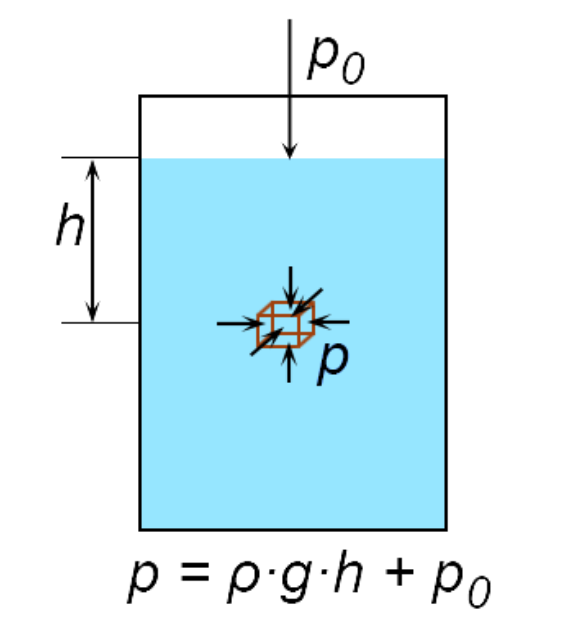
\includegraphics[width=0.4\textwidth]{Images/Kapittel4:Fluiddynamikk/hydro1.png} 
    \caption{Hydrostatisk trykk \( p \) i en væske, som avhenger av væskens tetthet \( \rho \), tyngdeakselerasjonen \( g \), dybden \( h \), og det ytre trykket \( p_0 \). Trykket øker jevnt med dybden.}
    \label{fig:hydro1}
\end{figure}

\begin{figure}[H]
    \centering
    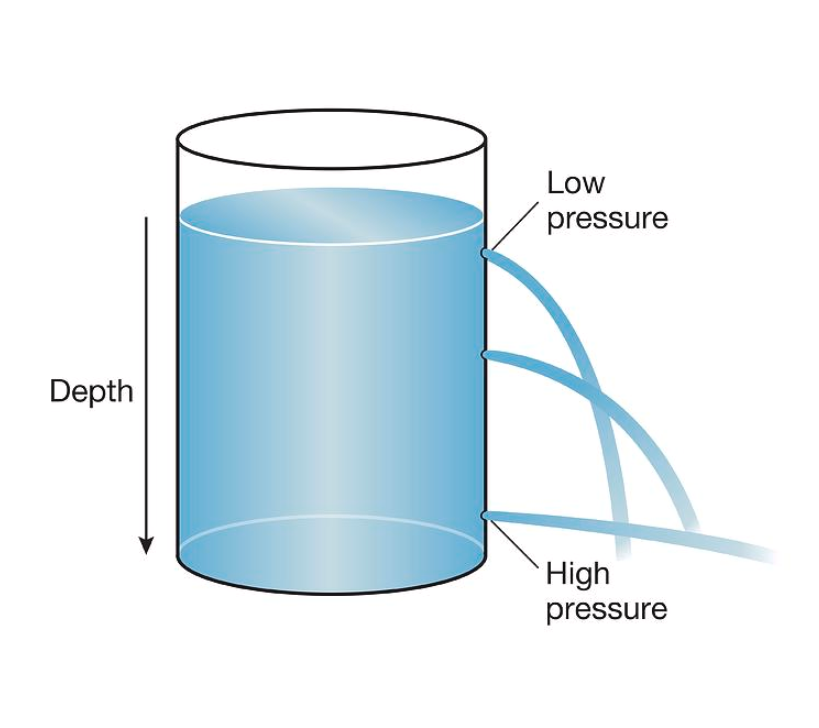
\includegraphics[width=0.7\textwidth]{Images/Kapittel4:Fluiddynamikk/hydrostatisk2.png} 
    \caption{Illustrasjon av trykk i en væske som øker med dybden. Ved større dybde er trykket høyere på grunn av vekten av væsken over punktet. Dette demonstreres av vannstrålene som går lenger ut jo dypere det er.}
    \label{fig:hydro2}
\end{figure}

\exm{Beregning av trykk ved ulike dybder}{
En dykker er under vann med tetthet \( \rho = 1000 \, \text{kg/m}^3 \), og det atmosfæriske trykket ved overflaten er \( p_0 = 101325 \, \text{Pa} \). Hva er det totale trykket på dykkeren ved dybdene \( h = 2 \, \text{m} \), \( h = 5 \, \text{m} \), og \( h = 10 \, \text{m} \)? \\

\textit{Metode:}
Bruk formelen for trykk i væsken:
\[
p(h) = p_0 + \rho g h
\]
hvor \( p_0 = 101325 \, \text{Pa} \), \( \rho = 1000 \, \text{kg/m}^3 \), og \( g = 9.81 \, \text{m/s}^2 \). Vi setter inn de tre ulike dybdene én etter én. \\

\textbf{Ved \( h = 2 \, \text{m} \):}
\[
p(2) = 101325 + 1000 \cdot 9.81 \cdot 2 = 101325 + 19620 = 120945 \, \text{Pa}.
\]

\textbf{Ved \( h = 5 \, \text{m} \):}
\[
p(5) = 101325 + 1000 \cdot 9.81 \cdot 5 = 101325 + 49050 = 150375 \, \text{Pa}.
\]

\textbf{Ved \( h = 10 \, \text{m} \):}
\[
p(10) = 101325 + 1000 \cdot 9.81 \cdot 10 = 101325 + 98100 = 199425 \, \text{Pa}.
\]

\textit{Svar:}
Trykket på dykkeren ved \( h = 2 \, \text{m} \) er \( 120945 \, \text{Pa} \), ved \( h = 5 \, \text{m} \) er det \( 150375 \, \text{Pa} \), og ved \( h = 10 \, \text{m} \) er det \( 199425 \, \text{Pa} \).
}

\section{Pascals lov}

Når vi utøver et ytre trykk \( \Delta p \) på en væske som er i ro, vil trykket i hele væsken øke med samme beløp \( \Delta p \). Dette betyr at trykkøkningen er lik i alle retninger, uavhengig av væskens høyde. Selv om trykkøkningen er konstant, vil det totale trykket fortsatt variere med høyden på grunn av det hydrostatiske trykket.

\tips{Viktige punkter om Pascals lov}{
- Trykkøkningen \( \Delta p \) forplanter seg likt i hele væsken.  
- Det totale trykket i væsken kan uttrykkes som summen av trykkøkningen og det hydrostatiske trykket.  
- Pascals lov danner grunnlaget for hydrauliske systemer, der små krefter kan forsterkes ved å bruke større arealer.
}

\defn{Pascals lov i hydrauliske systemer}{
    Når trykk påføres en væske i ro, gjelder følgende forhold for krefter og arealer i et hydraulisk system:
    \begin{align}
        \frac{F_1}{A_1} = \frac{F_2}{A_2},
    \end{align}
    hvor \( F_1 \) og \( F_2 \) er kreftene på stemplene, og \( A_1 \) og \( A_2 \) er arealene deres.  
    \textit{Utledning:} Trykkøkningen \( \Delta p \) i væsken er lik for begge stemplene:
    \[
    \Delta p = \frac{F_1}{A_1} = \frac{F_2}{A_2}.
    \]
    Ved å omskrive får vi:
    \[
    F_2 = F_1 \cdot \frac{A_2}{A_1}.
    \]
    Dette viser at kraften \( F_2 \) på det større stempelet er proporsjonal med forholdet mellom arealene \( \frac{A_2}{A_1} \).
}



\begin{figure}[H]
    \centering
    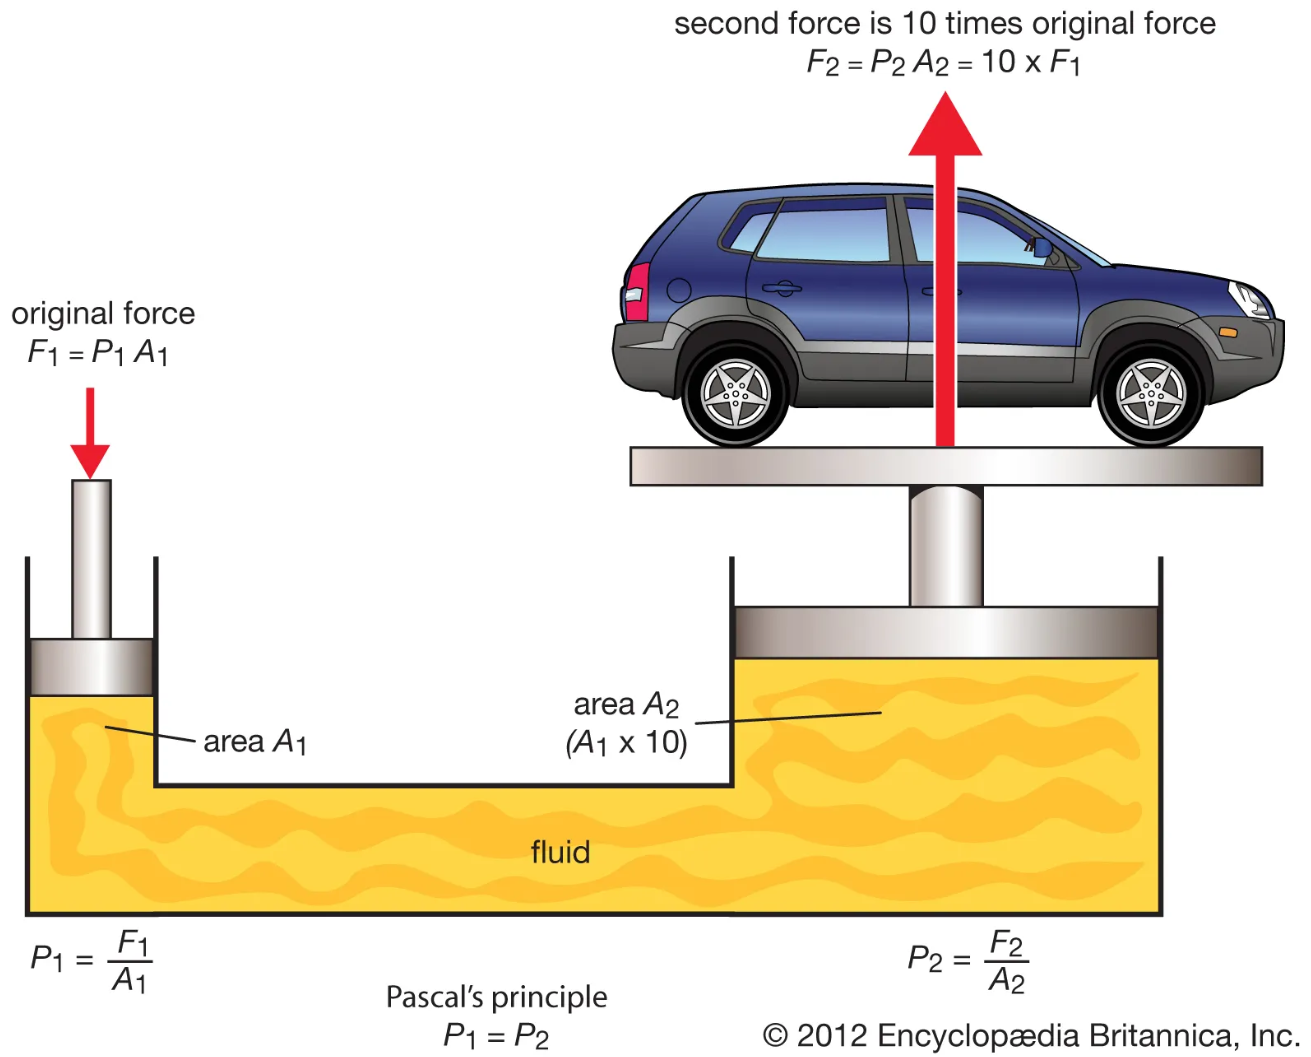
\includegraphics[width=0.8\textwidth]{Images/Kapittel4:Fluiddynamikk/pascals lov.png} 
    \caption{Pascals lov i et hydraulisk system. En liten kraft \( F_1 \) påføres et lite stempel med areal \( A_1 \), og skaper et trykk som forplanter seg gjennom væsken. Dette trykket løfter en bil ved å bruke et større stempel med areal \( A_2 \), som resulterer i en større kraft \( F_2 \).}
    \label{fig:pascalslov}
\end{figure}



\exm{Hydraulisk jekk}{%
En hydraulisk jekk har to stempler. Det lille stempelet har areal
$A_1 = \SI{5{,}0}{\centi\metre\squared} = \SI{5{,}0e-4}{\metre\squared}$
og det store stempelet har areal
$A_2 = \SI{200}{\centi\metre\squared} = \SI{2{,}0e-2}{\metre\squared}$.
En kraft $F_1 = \SI{50}{\newton}$ påføres det lille stempelet.

\begin{center}
\begin{tikzpicture}[scale=0.95, >={Stealth[length=5pt,width=4pt]}]
  % Left cylinder (small)
  \draw[thick] (0,0) rectangle (0.7, 1.5);
  % Right cylinder (large)
  \draw[thick] (1.5,0) rectangle (4.5, 1.5);
  % Connecting base
  \draw[thick] (0,0) -- (4.5,0);
  % Fluid fill
  \fill[defscol!15] (0.05,0.05) rectangle (0.65,0.7);
  \fill[defscol!15] (1.55,0.05) rectangle (4.45,0.7);
  % Left piston
  \fill[gray!50] (0.05,0.65) rectangle (0.65,0.85);
  % Right piston
  \fill[gray!50] (1.55,0.65) rectangle (4.45,0.85);
  % Force arrow left
  \draw[->, very thick, red!70!black] (0.35, 2.0) -- (0.35, 0.87)
      node[midway, right, font=\footnotesize] {$F_1$};
  % Force arrow right (up, larger)
  \draw[->, very thick, headCol] (3.0, 0.87) -- (3.0, 2.5)
      node[midway, right, font=\footnotesize] {$F_2$};
  % Area labels
  \node[font=\footnotesize, gray!60!black] at (0.35, -0.3) {$A_1$};
  \node[font=\footnotesize, gray!60!black] at (3.0, -0.3) {$A_2$};
\end{tikzpicture}
\end{center}

\noindent Hva er kraften $F_2$ som løfter på det store stempelet?

Fra Pascals lov er trykket likt på begge sider:
\[
  \frac{F_1}{A_1} = \frac{F_2}{A_2}
  \implies
  F_2 = F_1 \cdot \frac{A_2}{A_1}
      = \SI{50}{\newton} \cdot \frac{\SI{2{,}0e-2}{\metre\squared}}{\SI{5{,}0e-4}{\metre\squared}}
      = \doubleunderline{\SI{2000}{\newton}}
\]
Med et lite stempel kan vi altså løfte en last som er 40 ganger så tung — det er prinsippet bak bilheis og hydrauliske bremser.
}

\section{Oppdrift og Arkimedes' lov}

Når et legeme er omgitt av en væske, utøves en oppdriftskraft på legemet. Denne kraften skyldes forskjellen i trykk mellom væskens underside og overside av legemet. Oppdriftskraften \( O \) er direkte knyttet til vekten av væsken som fortrenges av legemet.

\subsection{Oppdriftskraft}
Forskjellen mellom trykkreftene på oversiden og undersiden av legemet gir en netto oppdriftskraft \( O \), som kan uttrykkes som:
\[
O = \rho_B g V_q
\]
hvor \( \rho_B \) er tettheten til væsken, \( g \) er tyngdeakselerasjonen, og \( V_q \) er volumet av væsken som fortrenges av legemet.

\defn{Oppdriftskraft}{
    Oppdriftskraften \( O \) på et legeme omgitt av en væske i ro kan uttrykkes som:
    \begin{align}
        O = \rho_B g V_q
    \end{align}
    Her er \( \rho_B \) tettheten til væsken, \( g \) er tyngdeakselerasjonen, og \( V_q \) er volumet av væsken som fortrenges av legemet.
}

\begin{figure}[H]
    \centering
    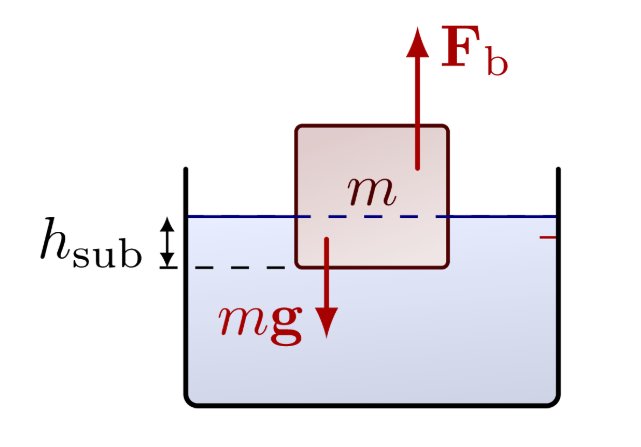
\includegraphics[width=0.5\textwidth]{Images/Kapittel4:Fluiddynamikk/oppdrift_h fortrengt.png} 
    \caption{Oppdrift \( F_b \), hvor oppdriftskraften beregnes ut fra volumet av væsken som fortrenges. Det fortrengte volumet er gitt som \( V_q = h_{\text{sub}} \cdot A \), der \( h_{\text{sub}} \) er dybden av den nedsenkede delen av legemet, og \( A \) er arealet av bunnflaten.}
    \label{fig:h-fortrengt}
\end{figure}


\subsection{Utledning fra trykkdifferanse}

Oppdriftskraften kan utledes direkte fra det hydrostatiske trykket.
Tenk deg et rektangulært legeme med grunnflate $A$ og høyde $h_s$, senket til dybde $h_1$ (topp) og $h_2 = h_1 + h_s$ (bunn):

\begin{center}
\begin{tikzpicture}[scale=0.90, >={Stealth[length=5pt,width=4pt]}]
  % Water surface
  \draw[dashed, gray!60] (-1.2, 2.5) -- (2.8, 2.5) node[right, font=\footnotesize, gray!60] {overflate};
  % Body
  \fill[headCol!20] (0.4, 0.6) rectangle (2.0, 1.9);
  \draw[thick] (0.4, 0.6) rectangle (2.0, 1.9);
  % Depth annotations
  \draw[<->, thin, gray!70] (-0.8, 2.5) -- (-0.8, 1.9)
      node[midway, left, font=\footnotesize] {$h_1$};
  \draw[<->, thin, gray!70] (-0.8, 2.5) -- (-0.8, 0.6)
      node[midway, right, font=\footnotesize] {$h_2$};
  % Force arrows
  \draw[->, very thick, defscol] (1.2, 1.9) -- (1.2, 2.6)
      node[above, font=\footnotesize] {$F_{\text{topp}}$};
  \draw[->, very thick, headCol] (1.2, 0.6) -- (1.2, -0.1)
      node[below, font=\footnotesize] {$F_{\text{bunn}}$};
  % Area label
  \node[font=\footnotesize] at (1.2, 1.25) {$A$};
\end{tikzpicture}
\end{center}

Trykkkraften \emph{ned} på toppen er $F_{\text{topp}} = p_1 \cdot A = (\rho_v g h_1)\,A$,
og kraften \emph{opp} på bunnen er $F_{\text{bunn}} = p_2 \cdot A = (\rho_v g h_2)\,A$.
Nettokraften oppover er:
\[
  O = F_{\text{bunn}} - F_{\text{topp}}
    = \rho_v g A (h_2 - h_1)
    = \rho_v g A h_s
    = \rho_v g V_{\text{fortrengt}}
\]
Dette er Arkimedes' lov, utledet fra hydrostatikk.

\subsection{Flyter eller synker?}

Nettokraften på et legeme med tetthet $\rho_L$ og volum $V$ i en væske med tetthet $\rho_v$ er:
\[
  F_{\text{netto}} = O - G = \rho_v g V - \rho_L g V = (\rho_v - \rho_L)\,g V
\]

\begin{tcolorbox}[colback=gray!13, colframe=gray!40, boxrule=0.5pt,
    arc=2pt, left=6pt, right=6pt, top=4pt, bottom=4pt]
\begin{itemize}
  \item $\rho_L < \rho_v$: $F_{\text{netto}} > 0$ — legemet \textbf{flyter} (akselererer opp til det er delvis ute av væsken).
  \item $\rho_L = \rho_v$: $F_{\text{netto}} = 0$ — legemet \textbf{svever} i likevekt inne i væsken.
  \item $\rho_L > \rho_v$: $F_{\text{netto}} < 0$ — legemet \textbf{synker}.
\end{itemize}
\end{tcolorbox}

\merk{Stål flyter ikke i vann — men et stålskip gjør det!}{%
Stål har tetthet $\rho \approx \SI{7850}{\kilo\gram\per\metre\cubed}$, langt høyere enn vann.
Likevel flyter et skip laget av stål, fordi \emph{skipet som helhet} — stål pluss luft inni —
har en gjennomsnittlig tetthet \emph{lavere} enn vann.
Det er den totale massen delt på det totale volumet som avgjør.}

\subsection{Gravitasjonskraft på et legeme}
Gravitasjonskraften \( G \) som virker på et legeme, avhenger av legemets masse \( m \) og tyngdeakselerasjonen \( g \). Hvis massen til legemet uttrykkes som \( m = \rho_L V \), der \( \rho_L \) er legemets tetthet og \( V \) er volumet, kan gravitasjonskraften skrives som:
\[
G = m g = \rho_L V g.
\]

\subsection{Arkimedes' lov}
Arkimedes' lov gir en generell beskrivelse av oppdriftskraften og sier:
\textit{Oppdriftskraften på et legeme i en væske i ro er lik vekten av den fortrengte væsken.}

\defn{Arkimedes' lov}{
    Oppdriftskraften \( O \) på et legeme i væske i ro kan skrives som:
    \begin{align}
        O = G_B
    \end{align}
    hvor \( G_B = \rho_B g V_q \) er vekten av den fortrengte væsken.
}

\exm{Oppdrift på en båt}{
En båt har et volum på \( V = 9.0 \, \text{m}^3 \), og \( 12\% \) av dette volumet er under vann.

\textbf{a) Hva er oppdriftskraften på båten?}

\textit{Metode:}  
Volumet av vann som fortrenges er:
\[
V_q = 0.12 \cdot V = 0.12 \cdot 9.0 = 1.08 \, \text{m}^3.
\]
Oppdriftskraften beregnes ved å bruke formelen for oppdrift:
\[
O = \rho_B g V_q = 1000 \cdot 9.81 \cdot 1.08 = 10594.8 \, \text{N}.
\]
Rundt av til:
\[
O \approx 11 \, \text{kN}.
\]

\textbf{b) Hva veier båten?}

\textit{Metode:}  
Når båten flyter, er oppdriftskraften lik tyngdekraften på båten. Tyngdekraften på båten kan skrives som:
\[
G = m g = \rho_L V g.
\]
Løs for massen \( m \):
\[
m = \frac{O}{g} = \frac{10594.8}{9.81} \approx 1080 \, \text{kg}.
\]

\textit{Svar:}  
Oppdriftskraften på båten er \( 11 \, \text{kN} \), og vekten av båten er \( 1080 \, \text{kg} \).
}









